%
% 5-sobolevraum.tex
%
% (c) 2022 Prof Dr Andreas Müller, OST Ostschweizer Fachhochschule
%
\section{Sobolev-Räume
\label{buch:skalarprodukt:section:sobolev}}
\kopfrechts{Sobolev-Räume}
Im Beispiel~\ref{buch:skalarprodukt:hilbertraum:bsp:sinreihe} haben 
wir eine Reihe kennengelernt, deren Partialsummen alle stetig sind,
da sie trigonometrische Polynome sind.
Doch die Grenzfunktion ist die Rechteckfunktion, die ganz offensichtlich
nicht stetig sind.
Die Norm des Hilbert-Raums $L^2$ ist offenbar nicht stark genug, die
Stetigkeit der Grenzfunktion sicherzustellen.

%
% tikztemplate.tex -- template for standalon tikz images
%
% (c) 2021 Prof Dr Andreas Müller, OST Ostschweizer Fachhochschule
%
\documentclass[tikz]{standalone}
\usepackage{amsmath}
\usepackage{times}
\usepackage{txfonts}
\usepackage{pgfplots}
\usepackage{csvsimple}
\usepackage{ifthen}
\usetikzlibrary{arrows,intersections,math}
\begin{document}
\def\skala{1}
\newboolean{draft}
\setboolean{draft}{false}
\begin{tikzpicture}[>=latex,thick,scale=\skala]

% add image content here
\def\s{12/(2*3.14159)}
\def\punkt#1#2{({(#1)*\s},{(#2)*\s})}

\draw[->] (-0.6,0) -- (13.2,0) coordinate[label={$x$}];
\draw[->] (0,{-1.72*\s}) -- (0,{1.8*\s}) coordinate[label={right:$y$}];

\begin{scope}
\clip (-0.6,{-1.8*\s}) rectangle (13.0,{1.8*\s});
\draw[color=blue] plot[domain=-20:420,samples=100]
	({(\x/360)*\s*2*3.14159},{(4/3.14159)*sin(\x)*\s});
\draw[color=blue] plot[domain=-20:420,samples=1000]
	({(\x/360)*\s*2*3.14159},{(4/3.14159)*(sin(\x)-sin(3*\x)/3)*\s});
\ifthenelse{\boolean{draft}}{}{
\draw[color=blue] plot[domain=-20:420,samples=1000]
	({(\x/360)*\s*2*3.14159},{(4/3.14159)*(sin(\x)-sin(3*\x)/(3*3)+sin(5*\x)/(5*5))*\s});
\draw[color=blue] plot[domain=-20:420,samples=1000]
	({(\x/360)*\s*2*3.14159},{(4/3.14159)*(sin(\x)-sin(3*\x)/(3*3)+sin(5*\x)/(5*5)-sin(7*\x)/(7*7))*\s});
\draw[color=blue] plot[domain=-20:420,samples=1000]
	({(\x/360)*\s*2*3.14159},{(4/3.14159)*(sin(\x)-sin(3*\x)/(3*3)+sin(5*\x)/(5*5)-sin(7*\x)/(7*7)+sin(9*\x)/(9*9))*\s});
\draw[color=blue] plot[domain=-20:420,samples=1000]
	({(\x/360)*\s*2*3.14159},{(4/3.14159)*(sin(\x)-sin(3*\x)/(3*3)+sin(5*\x)/(5*5)-sin(7*\x)/(7*7)+sin(9*\x)/(9*9)-sin(11*\x)/(11*11))*\s});
\draw[color=blue] plot[domain=-20:420,samples=1000]
	({(\x/360)*\s*2*3.14159},{(4/3.14159)*(sin(\x)-sin(3*\x)/(3*3)+sin(5*\x)/(5*5)-sin(7*\x)/(7*7)+sin(9*\x)/(9*9)-sin(11*\x)/(11*11)+sin(13*\x)/(13*13))*\s});
\draw[color=blue] plot[domain=-20:420,samples=1000]
	({(\x/360)*\s*2*3.14159},{(4/3.14159)*(sin(\x)-sin(3*\x)/(3*3)+sin(5*\x)/(5*5)-sin(7*\x)/(7*7)+sin(9*\x)/(9*9)-sin(11*\x)/(11*11)+sin(13*\x)/(13*13)-sin(15*\x)/(15*15))*\s});
\draw[color=blue] plot[domain=-20:420,samples=1000]
	({(\x/360)*\s*2*3.14159},{(4/3.14159)*(sin(\x)-sin(3*\x)/(3*3)+sin(5*\x)/(5*5)-sin(7*\x)/(7*7)+sin(9*\x)/(9*9)-sin(11*\x)/(11*11)+sin(13*\x)/(13*13)-sin(15*\x)/(15*15)+sin(17*\x)/(17*17))*\s});
\draw[color=blue] plot[domain=-20:420,samples=1000]
	({(\x/360)*\s*2*3.14159},{(4/3.14159)*(sin(\x)-sin(3*\x)/(3*3)+sin(5*\x)/(5*5)-sin(7*\x)/(7*7)+sin(9*\x)/(9*9)-sin(11*\x)/(11*11)+sin(13*\x)/(13*13)-sin(15*\x)/(15*15)+sin(17*\x)/(17*17)-sin(19*\x)/(19*19))*\s});
}
\end{scope}

\begin{scope}
	\clip (-0.6,{-1.8*\s}) rectangle (13.0,{1.8*\s});
	\draw[color=red,line width=1pt]
		\punkt{-0.5*3.14159}{-0.5*3.14159}
		--
		\punkt{0.5*3.14159}{0.5*3.14159}
		--
		\punkt{1.5*3.14159}{-0.5*3.14159}
		--
		\punkt{2.5*3.14159}{0.5*3.14159};
\end{scope}

\node at \punkt{0}{0} [below right] {$0\mathstrut$};
\node at \punkt{0.5*3.14159}{0} [below] {$\frac{\pi}2\mathstrut$};
\node at \punkt{3.14159}{0} [below left] {$\pi\mathstrut$};
\node at \punkt{1.5*3.14159}{0} [below] {$\frac{3\pi}2\mathstrut$};
\node at \punkt{2*3.14159}{0} [below right] {$2\pi\mathstrut$};

\foreach \x in {0.5,1,1.5,2}{
	\draw \punkt{\x*3.14159}{(0.05)} -- \punkt{\x*3.14159}{(-0.05)};
}
\draw \punkt{-0.05}{-0.5*3.14159} -- \punkt{0.05}{-0.5*3.14159};
\draw \punkt{-0.05}{0.5*3.14159} -- \punkt{0.05}{0.5*3.14159};
\draw \punkt{-0.05}{1} -- \punkt{0.05}{1};
\draw \punkt{-0.05}{-1} -- \punkt{0.05}{-1};
\node at \punkt{0}{-0.5*3.14159} [left] {$-\frac{\pi}2\mathstrut$};
\node at \punkt{0}{-1} [left] {$-1\mathstrut$};
\node at \punkt{0}{1} [left] {$1\mathstrut$};
\node at \punkt{0}{0.5*3.14159} [left] {$\frac{\pi}2\mathstrut$};


\end{tikzpicture}
\end{document}

%
Die Supremumnorm ist zwar stärker, gleichmässig konvergente Folgen
von stetigen Funktionen konvergieren gegen einen stetigen Grenzwert.
Aber sie ist ebenfalls nicht stark genug, um Differenzierbarkeit zu erzwingen.
Die Reihe
\begin{equation}
f(x)
=
\frac{4}{\pi}\biggl(
\sin x - \frac{\sin 3x}{3^2} + \frac{\sin 5x}{5^2} -\frac{\sin 7x}{7^2} +\dots
\biggr)
\label{buch:skalarprodukt:sobolevraum:eqn:fourierdreieck}
\end{equation}
hat beliebig oft stetig differenzierbare Partialsummen und sie konvergiert
gleichmässig gegen die stetige, aber an den Stellen $k\frac{\pi}2$,
$k\in\mathbb{Z}$, nicht differenzier Dreicksfunktion (siehe
Abbildung~\ref{buch:skalarprodukt:sobolevraum:fig:fourierdreieck}).

Die Beispiele zeigen, dass Stetigkeits- und Differenzierbarkeitseigenschaften
beim Arbeiten in einem Hilbert-Raum verloren gehen könnten.
Andererseits möchte man einen Hilbert-Raum dazu verwenden,
Differentialgleichungen zu lösen, wo man aus der Theorie weiss, dass
die Lösungen beliebig oft stetig differenzierbar sind.
Es ist daher anzunehmen, dass wir diese als Grenzfunktionen bezüglich
einer stärkeren Norm erhalten können, welche die Differenzierbarkeit
garantiert.
In diesem Abschnitt sollen die wesentlichen Ideen der Konstruktion
dieser sogenannten Sobolev-Räume skizziert werden.

%
% Skalaraprodukt mit Ableitungen
%
\subsection{Skalarprodukt mit Ableitungen}
So wie es einfach ist, die Stetigkeit der Grenzfunktion mit Hilfe
der Supremumnorm zu erzwingen, kann man ähnliche Normen mit den
Ableitungen definieren, zum Beispiel die Norm
\begin{equation}
\|f\|_{C^n}
=
\sup_{x\in [a,b]}\sup_{k\le n} \biggl|\frac{d^kf}{dx^k}(x)\biggr|,
\label{buch:skalarprodukt:sobolevraum:norm}
\end{equation}
die die Werte aller Ableitungen bis zur $k$-ten Ableitung berücksichtigt.
Eine Cauchy-Folge in dieser Norm ist auch eine Cauchy-Folge in der
Supremumnorm, die Grenzfunktion ist also stetig.
Für $k\le n$ ist aber auch die $k$-te Ableitung eine Cauchy-Folge
in der Supremumnorm, es konvergiert also auch die Folge der $k$-ten
Ableitungen gegen eine stetige Funktione.
Die Norm~\eqref{buch:skalarprodukt:sobolevraum:norm} stellt somit sicher,
dass Cauchy-Folgen gegen $n$-mal stetig differenzierbare Funktionen
konvergieren.

Die Norm~\eqref{buch:skalarprodukt:sobolevraum:norm} lässt sich aber
nicht aus einem Skalarprodukt ableiten.
Das hat zur Folge, dass es schwierig ist, Funktionen als Linearkombinationen
von Basisvektoren zusammenzusetzen.
Dafür ist es nötig, ein Skalarprodukt zu verwenden, welches ebenfalls
gross wird, wenn die Ableitungen der Funktion gross sind.

\begin{definition}[$W^{1,2}$-Skalarprodukt]
Seien $f$ und $g$ stetig differenzierbare Funktionen auf dem Intervall
$[a,b]$, dann ist
\begin{equation}
\langle f,g\rangle_{W^{1,2}}
=
\int_a^b \overline{f(x)} g(x)\,dx
+
\int_a^b \overline{f'(x)} g'(x)\,dx
=
\langle f, g\rangle
+
\langle f',g'\rangle
\label{buch:skalarprodukt:sobolevraum:eqn:W12produkt}
\end{equation}
ein Skalarprodukt.
\end{definition}

Es ist nachzuprüfen, dass $\langle\;\,,\;\rangle_{W^{1,2}}$ tatsächlich ein
Skalarprodukt ist.
Zunächst ist klar, dass $\langle\;\,,\;\rangle_{W^{1,2}}$ konjugiert
symmetrisch.
Es ist auch positiv definit, denn für eine Funktion $f\ne 0$
ist
\[
\langle f,f\rangle_{W^{1,2}}
=
\langle f,f\rangle + \langle f',f'\rangle
\ge
\|f\|^2
\ge
0.
\]
Es ist also nur noch zu überprüfen, dass $\langle\;\,,\;\rangle_{W^{1,2}}$ 
sesquilinear ist:
\begin{align*}
\langle f,\lambda g_1+\mu g_2\rangle_{W^{1,2}}
&=
\langle f,\lambda g_1+\mu g_2\rangle + \langle f',\lambda g_1'+\mu g_2'\rangle
=
\lambda \langle f,g_1\rangle
+
\mu \langle f,g_2\rangle
+
\lambda \langle f',g_1'\rangle
+
\mu \langle f',g_2'\rangle
\\
&=
\lambda \langle f,g_1\rangle_{W^{1,2}}
+
\mu \langle f,g_2\rangle_{W^{1,2}}.
\end{align*}
Konjugierte Linearität im ersten Argument folgt aus der Linearität
im zweiten Argument und der hermiteschen Symmetrie.

Aus dem Skalarprodukt $\langle\;\,,\;\rangle_{W^{1,2}}$ entsteht jetzt
die Norm
\begin{equation}
\|f\|_{W^{1,2}}^2
=
\int_a^b |f(x)|^2 + |f'(x)|^2 \,dx.
\label{buch:skalarprodukt:sobolevraum:eqn:w12norm}
\end{equation}
Die $L^2$-Norm einer Funktion in $C^1$ ist immer nach oben beschränkt
durch die Norm $\|f\|_{W^{1,2}}$.
Eine Cauchy-Folge $f_n$ in der Norm $\normfunc_{W^{1,2}}$ ist also
automatisch eine Cauchy-Folge in der gewöhnlichen $L^2$-Norm, sie
konvergiert also gegen eine Funktion $f=\lim_{n\to\infty} f_n \in L^2([a,b])$.
Gleichzeitig ist die Folge $f_n'$ ebenfalls eine Cauchy-Folge
in $L^2([a,b])$, es gibt also eine Funktion $f'\in L^2([a,b])$,
die Grenzfunktion der Folge $f_n'$ ist: $\lim_{n\to\infty} f_n' = f'$
in $L^2([a,b])$.
Der Grenzwert einer $L^2$-Folge ist nicht notwendigerweise eine
stetige Funktion, die Norm kann also nicht garantieren, dass die
Grenzwertfunktion $f$ überhaupt differenzierbar ist.
Es ist also nicht zulässig zu sagen, dass $f'$ die Ableitung von $f$
ist, aber sie verhält sich als Faktor in Integralen wie die Ableitung
von $f$.

Der Raum $C^1([a,b])$ der stetig differenzierbaren Funktionen mit
dem Skalarprodukt ist ein Prähilbertraum, durch Vervollständigung mit
allen Grenzwerten von Cauchy-Folgen entsteht ein Hilbert-Raum.

\begin{definition}[Sobolev-Raum]
Der Sobolev-Raum $W^{1,2}([a,b])$ ist die Vervollständigung des
\index{Sobolev-Raum}%
Prähilbertraumes $C^1([a,b])$ der differenzierbaren Funktionen auf
dem Intervall $[a,b]$ mit dem Skalarprodukt
\begin{equation}
\langle f,g\rangle_{W^{1,2}}
=
\int_a^b \overline{f(x)}g(x) + \overline{f'(x)}g'(x)\,dx.
\label{buch:skalarprodukt:sobolevraum:eqn:w12skalar}
\end{equation}
\end{definition}

Der Sobolev-Raum $W^{1,2}$ ist also der natürliche Raum, in dem
Aufgabenstellungen, bei denen es nicht nur auf Integrale, sondern
auch auf erste Ableitungen ankommt, bearbeitet werden können.

%
% Höhere Ableitungen
%
\subsection{Höhere Ableitungen}
Das Skalarprodukt~\eqref{buch:skalarprodukt:sobolevraum:eqn:w12skalar}
hat dabei geholfen, einen Hilbert-Raum von Funktionen zu konstruieren,
mit dem erste Ableitungen behandelt werden können.
Leider reicht das noch nicht, um höhere Ableitungen zu behandeln oder
Definitionsgebiete höherer Dimension also nur einfache Intervalle.
Im Folgenden sei also $\Omega\subset\mathbb{R}^n$ ein $n$-dimensionales
Gebiet.
Wir bezeichnen die Koordinaten mit $x_1,\dots,x_n$.

\subsubsection{Multiindizes und höhere Ableitungen}
Eine $k$-mal stetig differenzierbare Funktion $f\colon\Omega\to \mathbb{R}$ 
hat die partiellen ersten Ableitungen
\[
\frac{\partial f}{\partial x_1},
\dots,
\frac{\partial f}{\partial x_n}.
\]
Für höhere partielle Ableitungen wird diese Notation sehr schwerfällig.
Die mehrfache Ableitung von $f$, die $k_i$-fach nach der Variablen $x_i$
abgeleitet ist, wird
\[
\frac{
\partial^{k_1+k_2+\dots+k_n} f
}{
\partial x_1^{k_1}\,\partial x_2^{k_2} \dots \partial x_n^{k_n}
}
\]
geschrieben.
Die Ordnung der Ableitung ist $k_1+k_2+\dots+k_n$.
Die Ableitung ist offensichtlich durch die natürlichen Zahlen
$(k_1,\dots,k_n)$ definiert.
Dies führt auf die folgende, schlankere Notation.

\begin{definition}[Multiindex]
Ein Element $\bm{k}\in \mathbb{N}^n$ heisst ein $n$-dimensionaler
{\em Multiindex} der Ordnung $|\bm{k}|= k_1+\dots+k_n$.
\index{Multiindex}%
\end{definition}

Mit Multiindizes lassen sich jetzt viele Operationen, die bei
Funktionen mit mehreren Variablen häufig auftauchen, sehr elegant
abkürzen.

\begin{itemize}
\item Gleichheit:
$\bm{k}=\bm{l}\;\Leftrightarrow\; k_1=l_1\wedge\dots\wedge k_n=l_n$.
\item Vergleich:
$\bm{k}\le \bm{l}\;\Leftrightarrow\; k_1\le l_1\wedge\dots\wedge k_n\le l_n$.
\item Summe:
$\bm{k}+\bm{l} = \bm{m}
\;\Leftrightarrow\;
m_i=k_i+l_i,\; i = 1,\dots,n$.
\item Fakultät: $\bm{k}! = k_1!\cdots k_n!$
\item Multinomialkoeffizient:
\(
\displaystyle
\binom{|\bm{k}|}{\bm{k}}
=
\frac{|\bm{k}|!}{\bm{k}!}
=
\frac{|\bm{k}|!}{k_1!\cdots k_n!}
\)
\item Potenz: Seien die Variablen $x=(x_1,\dots,x_n)$ gegeben, dann soll
\(
x^{\bm{k}} = x_1^{k_1}\cdot \ldots \cdot x_n^{k_n}
\)
bedeuten.
\item Ableitungen: Sei $f$ eine Funktion der Variablen $x_1,\dots,x_n$, dann
ist die $\bm{k}$-te Ableitung
\[
D^{\bm{k}}f(x_1,\dots,x_n)
=
D_1^{k_1}\dots D_n^{k_n} f(x_1,\dots,x_n)
=
\frac{
\partial^{|\bm{k}|}f
}{
\partial x_1^{k_1}\dots\partial x_n^{k_n}
}(x_1,\dots,x_n),
\]
darin ist $D_i=\partial/\partial_i$ die partielle Ableitung nach $x_i$.
\end{itemize}
Die Multiindex-Notation kann zum Beispiel verwendet werden, um die
Taylor-Polynome vom Grad $k$ einer Funktionen $f(x_1,\dots,x_n)$ von
$n$-Variablen zu formulieren.
Das Taylor-Polynome vom Grad $k$ im Punkt $(0,\dots,0)$ ist
\begin{align*}
\mathscr{T}^kf(x_1,\dots,x_n)
&=
\sum_{|\bm{k}|\le k} \frac{1}{\bm{k}!} D^{\bm{k}} f(0,\dots,0)\cdot x^{\bm{k}},
\intertext{in einem beliebigen Punkt $x^*=(x_1^*,\dots,x_n^*)$ ist es:}
\mathscr{T}^kf(x_1,\dots,x_n)
&=
\sum_{|\bm{k}|\le k} \frac{1}{\bm{k}!} D^{\bm{k}} f(x^*) \cdot (x-x^*)^{\bm{k}}.
\end{align*}

%
% Skalarprodukt
%
\subsubsection{Skalarprodukt}
Die Multiindexnotation ermöglich jetzt, auf sehr elegante Art und 
Weise ein Skalarprodukt für $k$-mal stetig differenzierbare Funktionen
zu definieren.

\begin{definition}[$W^{1,2}(\Omega)$-Skalarprodukt]
Seien $f$ und $g$ $k$-mal stetig differenzierbare Funktionen auf dem
Gebiet $\Omega$, dann ist
\[
\langle f,g\rangle_{W^{k,2}(\Omega)}
=
\int_\Omega
\sum_{|\bm{k}|\le k}
\overline{D^{\bm{k}}f(x)}
D^{\bm{k}}g(x)
\,dx
\]
das {\em $W^{k,2}(\Omega)$-Skalarprodukt}.
Die zugehörige {\em $W^{k,2}(\omega)$-Norm} ist
\[
\|f\|_{W^{k,2}(\Omega)}^2
=
\int_\Omega
\sum_{|\bm{k}|\le k}
|D^{\bm{k}}f(x)|^2
\,dx
\]
\end{definition}

Es ist aus der Definition unmittelbar klar, dass
$\langle\;\,,\;\rangle_{W^{k,2}(\Omega)}$
konjugiert symmetrisch ist.
Wie im eindimensionalen Fall kann man nachrechnen, dass 
$\langle\;\,,\;\rangle_{W^{k,2}(\Omega)}$
linear ist.
Dazu seien $f,g_1$ und $g_2$ $k$-fach stetig differenzierbare Funktionen
und $\lambda,\mu\in\mathbb{C}$.
Damit kann man berechnen
\begin{align*}
\langle f,\lambda g_1+\mu g_2\rangle_{W^{k,2}(\Omega)}
&=
\int_{\Omega}
\sum_{|\bm{k}|\le k}
\overline{D^{\bm{k}}f(x)}
D^{\bm{k}}(\lambda g_1(x)+\mu g_2(x))
\,dx
\\
&=
\lambda
\int_{\Omega}
\sum_{|\bm{k}|\le k}
\overline{D^{\bm{k}}f(x)}
\,D^{\bm{k}}g_1(x)
\,dx
+
\mu
\int_{\Omega}
\sum_{|\bm{k}|\le k}
\overline{D^{\bm{k}}f(x)}
\,D^{\bm{k}}g_2(x)
\,dx
\\
&=
\lambda
\langle f,g_1\rangle_{W^{k,2}(\Omega)}
+
\mu
\langle f,g_2\rangle_{W^{k,2}(\Omega)}.
\end{align*}
Wegen $\|f\|_{W^{k,p}(\Omega)}^2 \ge \|f\|_{L^2(\Omega)}$ ist 
$\langle\;\,,\;\rangle_{W^{k,2}(\Omega)}$ positiv definit und damit
ein Skalarprodukt.

%
% Sobolev-Raum 
%
\subsubsection{Der Sobolev-Raum $W^{k,2}(\Omega)$}
Der Vektorraum der $k$-mal stetig differenzierbaren Funktionen 
ist bezüglich der Norm $\normfunc_{W^{k,2}(\Omega)}$-Norm
ein Prähilbertraum, aber nicht vollständig.
Wenn $f_n$ eine Cauchy-Folge von $k$-mal stetig differenzierbaren
Funktionen in der $W^{k,2}(\Omega)$-Norm ist, dann ist $D^{\bm{k}}f$
für jeden Multiindex $|\bm{k}|\le k$ eine Cauchy-Folge in der
$L^2(\Omega)$-Norm.
Da $L^2(\Omega)$ ein Hilbert-Raum ist, gibt es für jeden Multiindex $\bm{k}$
eine Funktion $f^{\bm{k}}\in L^2(\Omega)$, die Grenzwert
\[
f^{(\bm{k})} = \lim_{n\to\infty} D^{\bm{k}}f(x)
\]
der Cauchy-Folge $D^{\bm{k}}f$ ist.
Wie im eindimensionalen Fall ist auch in $W^{k,2}(\Omega)$ nicht
sichergestellt, dass die Grenzfunktion differenzierbar ist, dass ein
Ausdruck wie $D^{\bm{k}}f(x)$ überhaupt sinnvoll ist.

\begin{definition}[Sobolev-Raum $W^{1,2}(\Omega)$]
Der Sobolev-Raum $W^{k,2}(\Omega)$ ist der Hilbert-Raum, der durch
Vervollständigung des Vektorraums der $k$-mal stetig differenzierbaren
Funktionen bezüglich der $W^{k,2}(\Omega)$-Norm entsteht.
\end{definition}

%
% Ableitungen
%
\subsection{Schwache Ableitung}
Die Diskussion der $W^{k,2}(\Omega)$-Norm hat gezeigt, dass es in diesem
erweiterten Funktionenraum nicht mehr sinnvoll sein kann, die Ableitung
als Grenzwert eines Differenzenquotienten zu definieren.
Nur für genügend oft stetig differenzierbare Funktionen ist diese
Definition praktikabel.

Die schwache Ableitung ist ein Ersatz, der sich an der Idee des
Skalarproduktes orientiert.
Sei $f\colon \Omega\to\mathbb{R}$ eine genügend oft differenzierbare
Funktion.
Statt die Ableitung direkt zu studieren untersuchen wir das Skalarprodukt
der Ableitung mit besonders einfach zu handhabenden Funktionen.
Diese Funktionen sollen keine Schwierigkeiten beim Ableiten
verursachen können, sie sollen also unendlich oft stetig differenzierbar
sein.
Der Wert der Ableitung einer Funktion in einem Punkt $x\in\Omega$ hängt nur 
von den Werten von $f$ in der unmittelbaren Umgebung dieses Punktes ab.
Wenn wir die Ableitung mit Hilfe eines Skalarproduktes testen wollen,
dann muss dies mit Funktionen möglich sein, die nur in unmittelbarer
Umgebung eines Punktes von $0$ verschieden sind.

Die Forderung, dass der Abschluss des Trägers einer Funktion $f$
in $\Omega$ kompakt ist, hat zur Folge, dass $f(x)=0$ überall auf dem Rand
von $\Omega$ und dies gilt auch für alle Ableitungen.

\begin{definition}[Testfunktion]
\index{Testfunktion}%
Die Menge $C_c^{\infty}(\Omega)$ der beliebig of stetig differenzierbar
Funktionen mit kompaktem Träger heisst die Menge der {\em Testfunktionen}.
\end{definition}

Sei jetzt $f$ eine $k$-mal stetig differenzierbare Funktion.
Wir möchten die Ableitung $D^{\bm{k}}f$ durch ihre Skalarprodukte mit
Testfunktionen charakterisieren.
Dazu betrachten wir das Skalarprodukt
\(
\langle D^{\bm{k}}f,\varphi\rangle
\)
mit einer Testfunktion $\varphi \in C_c^{\infty}$.
Da $\varphi$ beliebig oft differenzierbar ist, können wir
partielle Integration verwenden, um die Ableitung von $f$ auf $\varphi$
hinüberzuschieben.
Dabei treten Randterme an den Integrationsgrenzen auf.
Da $\varphi$ kompakten Träger hat, sind die Randwerte von $\varphi$
immer 0, die Randterme verschwinden daher.
Somit können wir berechnen:
\begin{align*}
\langle D^{\bm{k}}f,\varphi\rangle
&=
\int_{\Omega} \overline{D^{\bm{k}}f(x)}\, \varphi(x)\,dx
=
-\int_{\Omega}
\overline{D^{\bm{k}-(1,0,\dots,0)}f(x)}\, 
D_1 \varphi(x)
\,dx
= \dots
\\
&=
(-1)^{|\bm{k}|} \int_{\Omega} \overline{f(x)} \, D^{\bm{k}}\varphi(x) \,dx
=
(-1)^{|\bm{k}|} \langle f,D^{\bm{k}}\varphi\rangle.
\end{align*}
Die Rechnung zeigt, dass das Skalarprodukt mit der $\bm{k}$-ten
Ableitung durch die Skalarprodukt mit Ableitungen von Testfunktionen
charakterisiert werden kann.

\begin{definition}[schwache Ableitung]
Sei $f\colon\Omega\to\mathbb{R}$  eine integrierbare Funktion.
Wir sagen, eine integrierbare Funktion $v\colon\Omega\to\mathbb{R}$ 
ist eine {\em schwache $\bm{k}$-te Ableitung} von $f$ wenn 
\[
\langle v,\varphi\rangle
=
(-1)^{|\bm{k}|} \langle v,D^{\bm{k}}\varphi\rangle
\]
für alle Testfunktionen $\varphi C_c^{\infty}(\Omega)$ gilt.
\end{definition}

Man kann mit dem
Abbildungssatz~\ref{buch:skalarprodukt:hilbertraum:satz:riesz}
von Riesz zeigen, dass die schwache Ableitung einer Funktion
in $L^2$ eindeutig ist und dass viele der gewohnten Rechenregeln
sich auf schwache Ableitungen übertragen lassen.
Besonders wichtig dabei ist die Beobachtung, dass die Funktionen
in $W^{k,2}(\Omega)$ aus integrierbaren Funktionen besteht, die 
schwache Ableitungen vom Grad höchstens $k$ in $L^2$ haben.

\begin{beispiel}
\label{buch:skalarprodukt:sobolevraum:bsp:schwachexistiert}
%
% schwach.tex
%
% (c) 2023 Prof Dr Andreas Müller
%
\begin{figure}
\centering
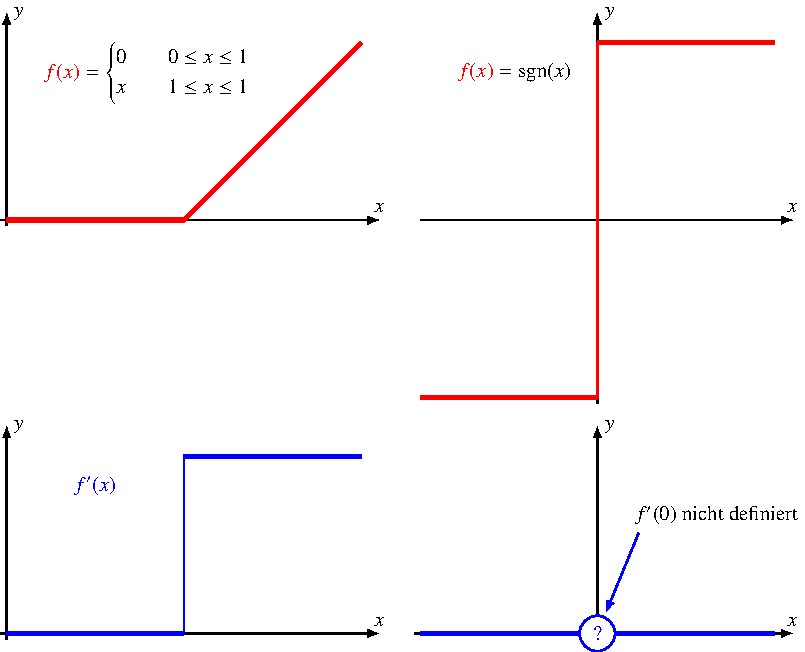
\includegraphics{chapters/010-skalarprodukt/images/schwach.pdf}
\caption{Schwache Ableitung einer nicht differenzierbaren Funktion.
Links die schwache Ableitung der Funktion von
Beispiel~\ref{buch:skalarprodukt:sobolevraum:bsp:schwachexistiert}.
Für die Signum-Funktion von
Beispiel~\ref{buch:skalarprodukt:sobolevraum:bsp:schwachexistiertnicht}
existiert die schwache Ableitung nicht, sie lässt für den Punkt $0$
nicht definieren.
\label{buch:skalarprodukt:sobolevraum:fig:schwach}}
\end{figure}
%
Die in Abbildung~\ref{buch:skalarprodukt:sobolevraum:fig:schwach} links
dargestellte Funktion
\[
f\colon (0,1) \to \mathbb{R}
:
x \mapsto
\begin{cases}
x&\qquad\text{für $0<x<1$}\\
1&\qquad\text{für $1\le x<2$}
\end{cases}
\]
ist stetig und integrierbar, aber sie ist an der Stelle $x=1$ nicht
differenzierbar.
Wir suchen die schwache Ableitung $v$ von $f$.

In einer Umgebung eines Punktes $x>1$ können wir Testfunktionen $\varphi$
so wählen, dass ihr Träger vollständig im Inneren des Intervals $(1,2)$
enthalten ist.
Mit diesen Testfunktionen können wir so rechnen, wie wenn $f$ die konstante
Funktion $1$ ist.
Das bedeutet für das Skalarprodukt
\[
\langle f,\varphi'\rangle
=
\int_1^2 \varphi'(x)\,dx
=
[\varphi(x)]_0^1 = 0.
\]
Das Skalarprodukt mit jeder beliebigen Testfunktion ist $0$, wir
müssen also $v(x)=0$ wählen.

Für $x$ im Teilinterval $(0,1)$ können wir die Testfunktionen so wählen,
dass der Träger vollständig im Inneren  von $(0,1)$ enthalten ist und
somit $f$ als die beliebig oft stetig differenzierbare Funktion $x$
behandelt werden darf.
Für das Skalarprodukt folgt dann
\[
-\langle f,\varphi'\rangle
=
-\int_0^1 f(x)\,\varphi'(x)\,dx
=
-\int_0^1 x\varphi'(x)\,dx
=
-[x\varphi(x)]_0^1 +\int_0^1 \varphi(x)\,dx
=
\langle 1,\varphi(x)\rangle,
\]
in diesem Teil des Intervals muss die schwache Ableitung den Wert $1$ 
haben.

Wir haben somit gefunden, dass die schwache Ableitung von $f$ die
Funktion
\[
v(x) = \begin{cases}
1&\qquad\text{für $0\le x<1$}
\\
0&\qquad\text{für $1< x<2$}
\end{cases}
\]
ist.
Wir kontrollieren dies, indem wir das Skalarprodukt für beliebige 
Testfunktionen $\varphi$ nachrechnen:
\begin{align*}
\langle v,\varphi\rangle
&=
\int_0^2 v(x)\,\varphi(x)\,dx
=
\int_0^1 1\,\varphi(x)\,dx
+
\int_1^2 0\,\varphi(x)\,dx.
\intertext{Jedes dieser Integrale kann man partiell integrieren:}
&=
[x\varphi(x)]_0^1 - \int_0^1 x\varphi'(x)\,dx
+
[1\varphi(x)]_1^2 - \int_1^2 1\varphi'(x)\,dx
\\
&=
\varphi(1) + \varphi(2) - \varphi(1) - \int_0^2 f(x)\,\varphi'(x)\,dx.
\intertext{Da $2$ ein Randpunkt ist, ist $\varphi(2)=0$, so dass sich}
&=-\langle f,\varphi'\rangle.
\end{align*}
ergibt.
Die Funktion $v$ ist also die schwache Ableitung von $f$.
\end{beispiel}

Eine Funktion in $W^{1,2}(\Omega)$ hat eine schwache Ableitung,
wie das Beispiel gezeigt hat, muss die Ableitung keine stetige
Funktion sein.
Ausserdem ist jede andere Funktion, die sich von der schwachen
Ableitung auf einer Menge vom Mass 0 unterscheidet, genauso eine
schwache Ableitung.
Trotzdem kann eine Funktion mit einer schwachen Ableitung nicht
beliebig ``wild'' sein, wie das folgende Beispiel zeigt.

\begin{beispiel}
\label{buch:skalarprodukt:sobolevraum:bsp:schwachexistiertnicht}
Die Signum-Funktion
\[
f\colon (-1,1) = \operatorname{sgn}(x) =
\begin{cases}
         - 1&\qquad\text{für $-1<x<0$}\\
\phantom{-}0&\qquad\text{für $x=0$}\\
\phantom{-}1&\qquad\text{für $0<x<1$}
\end{cases}
\]
ist nicht stetig (Abbildung~\ref{buch:skalarprodukt:sobolevraum:fig:schwach}).
$f$ ist fast überall konstant, in beiden Teilintervallen $(-1,0)$ und
$(0,1)$ ist die einzige mögliche schwache Ableitung von $f$ die
Nullfunktion.
Trotzdem kann $0$ nicht die schwache Ableitung von $f$ sein.
Wir wählen eine Testfunktion $\varphi$, die im Punkt $x=0$ von
Null verschieden ist.
Wäre $v$ eine schwache Ableitung von $f$, dann müsste
\begin{align*}
\langle v,\varphi\rangle
&=
-\langle f,\varphi'\rangle
=
-\int_{-1}^1 f(x) \varphi'(x)\,dx
\\
&=
-\int_{-1}^0 (-1)\cdot \varphi'(x)\,dx
-\int_{0}^1 1\cdot \varphi'(x)\,dx
=
\int_{-1}^0 \varphi'(x)\,dx
-
\int_{0}^1 \varphi'(x)\,dx
\\
&=
[\varphi(x)]_{-1}^0
-
[\varphi(x)]_{0}^1
=
\varphi(0)-\varphi(-1)
-
\varphi(1)+\varphi(0)
\\
&=
2\varphi(0)
\ne 0.
\end{align*}
Andererseits ist die Nullfunktion der einzige Kandidat für die
schwache Ableitun, für die das Skalarprodukt $\langle v,\varphi\rangle=0$
ist.
Dieser Widerspruch zeigt, dass die Funktion $f$ kein schwache
Ableitung hat.
\end{beispiel}

Die schwache Ableitung ermöglicht also mit gewissen Funktionen zu arbeiten,
die keine Ableitung im traditionellen Sinne haben.
Dank der Definition mit Hilfe eines Skalarproduktes in einem 
Hilbert-Raum darf man sich die Funktionen als Grenzwerte von
Cauchy-Folgen vorstellen.

%
% Physikalische Rechtfertigung
%
\subsection{Physikalische Rechtfertigung der schwachen Ableitung}
Die schwache Ableitung ersetzt die mit Hilfe eines Differenzenquotienten
definierte Änderungsrate durch eine Änderungsrate, die durch Vergleich
mit einer in der Umgebung eines Punktes konzentrierten Testfunktion
ermittelt wird.
Auf den ersten Blick mag das als Konzession an die Präzision der Ideen
der Analysis erscheinen, die Newton erfunden hat, um die Physik auf eine
neue Grundlage zu stellen.
Dabei wird aber vergessen, dass der Differenialquotient eine physikalisch
nicht erreichbare Idealisierung darstellt.
Keine Messung kann in einem Punkt im geometrischen Sinn erfolgen.
Die Bestimmung einer Position eines Massepunktes zum Beispiel erfolgt
durch Beobachtung des Lichtes, das vom Massepunkt reflektiert wird.
Doch der Massepunkt ist kein Punkt im geometrischen Sinn, er ist ausgedehnt
über ein endliches Gebiet.
Auch ist die Messung nicht instantan, es wird Licht gemessen, welches
über ein Zeitintervall vom Massepunkt reflektiert wird.
Das Messresultat entsteht also notwendigerweise als Mittelwert der
Beobachtung einer sehr grossen Zahl von Photonen, die von verschiedenen
Stellen reflektiert wurden.
Ein solcher Mittelwert ist genau das, was ein Skalarprodukt
$\langle f,\varphi\rangle$ mit einer Testfunktion ermittelt.

Die Feldgleichungen der Elektrodynamik wurden von Maxwell ausgehend
von Faradays Ideen als partielle Differentialgleichungen formuliert.
Sie verknüpfen die Werte des elektrischen Feldes $\vec{E}$ und des
magnetischen Feldes $\vec{B}$ mit der Ladungsdichte $\varrho$
und der Stromdichte $\vec{\jmath}$, die die Felder erzeugen.
Doch sowohl die Ladungsdichte wie auch die Stromdichte sind Idealisierungen.
Ladungen und Ströme sind nicht stetig über den Raum verteilt, sondern 
in Elektronen oder Atomkernen konzentriert.
Die Ladungsdichte entsteht daraus durch Messung der Ladung in einem kleine
Raumgebiet und Mittelung, was man wieder als Skalarprodukt mit einer
Testfunktion beschreiben kann.

Das elektrische Feld wird gemessen, indem die Kraft auf eine Testladung
im Feld ermittelt wird.
Ausser den prinzipiellen Einschränkungen an die Genauigkeit der
Positionsmessung wissen wir auch aus der Quantenmechanik, dass so etwas
wie die exakte Position eines Teilchens nicht gibt, wir können nur eine
Wahrscheinlichkeitsverteilung dafür bekommen.
Die Kraft äussert sich in einer Geschwindigkeitsänderung, die aber erst
messbar wird, wenn man die Beschleunigung eine gewisse Zeit lang aufrecht
erhält.
Das Messresultat ist also wieder ein Mittelwert über viele Positionen
und Zeitpunkte, oder anders ausgedrückt ein Skalarprodukt mit einer
Testfunktion.

Weitere Beispiele kann man auch in der Fluiddynamik finden.
Die Navier-Stokes-Gleichungen beschreiben die Strömung eines Mediums
unter der Annahme, dass es durch die Dichte $\varrho$ und die
Geschwindigkeit exakt beschreiben lässt.
Das Medium setzt sich aber aus einzelnen Atomen zusammen, die Dichte
ist also bereits ein Mittelwertbildung.
Bei der Geschwindigkeit wird das Problem noch deutlicher.
Auch die Strömungsgeschwindigkeit eines Gases ist der Mittelwert der
Strömungsgeschwindigkeit der Teilchen. 
Die Geschwindigkeit einzelner Teilchen ist dabei meistens sehr viel
grösser, nämlich im Bereich der Schallgeschwindigkeit, und äussert sich
in der Temperatur des Gases, also der mittleren kinetischen Energie.
Es ist nicht sinnvoll, von der Temperatur eines einzelnen Atoms zu
sprechen.

Alle diese Beispiele zeigen, dass die Ableitung als Änderungsrate, die
mit einem Differenzenquotienten bestimmt werden kann, eine Idealisierung
ist.
Wir können dies sogar etwas formeller zeigen.
Sei $x(t)$ die Koordinate eines Massepunktes zur Zeit $t$.
Die Messung kann nicht instantan erfolgen, im besten Fall ist die
gemessene Position ein Integral der Form
\[
\hat{x}(t)
=
\int_{-\infty}^\infty x(\tau) \varphi(\tau - t)\,d\tau.
\]
Darin ist $\varphi$ eine Testfunktion mit Träger in der Nähe von $0$.
Schreiben wir $T_t\varphi(\tau) = \varphi(\tau -t)$, dann können wir
das Messresultat auch als Skalarprodukt
$\hat{x}(t)=\langle x,T_t\varphi\rangle$
schreiben.
Die Messung mit der gleichen Aparatur einen Moment $\Delta t$ später ergibt
\[
\hat{x}(t+\Delta t)
=
\int_{-\infty}^\infty x(\tau) \varphi(\tau-t-\Delta t)\,dt
=
\langle x, T_{t+\Delta t}\varphi\rangle.
\]
Die Geschwindigkeit als Differenzenquotient ist
\begin{equation}
\frac{
\hat{x}(t+\Delta t)-\hat{x}(t)
}{\Delta t}
=
\frac{
\langle f,T_{t+\Delta t}\varphi\rangle
-
\langle f,T_{t}\varphi\rangle
}{
\Delta t
}
=
\left\langle
f,\frac{T_{t+\Delta t}\varphi - \varphi}{\Delta t}
\right\rangle
\label{buch:skalarprodukt:sobolevlraum:eqn:geschwindigkeit}
\end{equation}
Die Funktion $(T_{t+\Delta t}\varphi-T_t\varphi)/\Delta t$ ist eine 
beliebig oft stetig differenzierbare Funktion, die im Grenzwert
$\Delta t\to 0$ gegen
\[
\frac{
\varphi(\tau - t - \Delta t)
-
\varphi(\tau - t)
}{
\Delta t
}
=
-
\frac{
\varphi(\tau - t + \delta) - \varphi(\tau - t)
}{
\delta
}
\to 
-
\varphi'(\tau - t)
\quad
\text{für $\delta = - \Delta \to 0$}
\]
konvergiert.
Der Differenzenquotient
\eqref{buch:skalarprodukt:sobolevlraum:eqn:geschwindigkeit}
konvergiert daher gegen
\[
\lim_{\Delta t\to 0}
\frac{
\hat{x}(t+\Delta t)-\hat{x}(t)
}{\Delta t}
=
\left\langle
x,
\lim_{\Delta t\to 0}
\frac{T_{t+\Delta t}\varphi-T_t\varphi}{\Delta t}
\right\rangle
=
\langle f,-\varphi'\rangle
=
-
\langle f, \varphi'\rangle.
\]
Dieses einfache Modell einer ``unscharfen'' Messung führt also automatisch
auf das Konzept der schwachen Ableitung.






